\documentclass[twoside,11pt]{article} 
\usepackage{amsmath,amsfonts,bm}
\usepackage{listings}
\lstset{language=Matlab}%代码语言使用的是matlab
\lstset{breaklines}%自动将长的代码行换行排版
\lstset{extendedchars=false}%解决代码跨页时,章节标题,页眉等汉字不显示的问题
\usepackage{hyperref}
\usepackage{pgf,tikz,pgfplots}
%\usepackage[active,tightpage]{preview}
%\PreviewEnvironment{tikzpicture}
%\setlength\PreviewBorder{5pt}
\usetikzlibrary{arrows}
\pagestyle{empty}
\usepackage{pstricks-add}
\usepackage{amsthm} 
\usepackage{amssymb}
\usepackage{framed,mdframed}
\usepackage{graphicx,color} 
\usepackage{mathrsfs,xcolor} 
\usepackage[all]{xy}
\usepackage{fancybox} 
\usepackage{xeCJK}
\newtheorem{adtheorem}{定理}
\setCJKmainfont[BoldFont=FangSong_GB2312,ItalicFont=FangSong_GB2312]{FangSong_GB2312}
\newenvironment{theorem}
{\begin{mdframed}[backgroundcolor=gray!40,rightline=false,leftline=false,topline=false,bottomline=false]\begin{adtheorem}}
    {\end{adtheorem}\end{mdframed}}
\newtheorem{bdtheorem}{定义}
\newenvironment{definition}
{\begin{mdframed}[backgroundcolor=gray!40,rightline=false,leftline=false,topline=false,bottomline=false]\begin{bdtheorem}}
    {\end{bdtheorem}\end{mdframed}}
\newtheorem*{cdtheorem}{习题}
\newenvironment{exercise}
{\begin{mdframed}[backgroundcolor=gray!40,rightline=false,leftline=false,topline=false,bottomline=false]\begin{cdtheorem}}
    {\end{cdtheorem}\end{mdframed}}
\newtheorem{ddtheorem}{注}
\newenvironment{remark}
{\begin{mdframed}[backgroundcolor=gray!40,rightline=false,leftline=false,topline=false,bottomline=false]\begin{ddtheorem}}
    {\end{ddtheorem}\end{mdframed}}
\newtheorem{edtheorem}{引理}
\newenvironment{lemma}
{\begin{mdframed}[backgroundcolor=gray!40,rightline=false,leftline=false,topline=false,bottomline=false]\begin{edtheorem}}
    {\end{edtheorem}\end{mdframed}}
% \usepackage{latexdef}
\def\ZZ{\mathbb{Z}} \topmargin -0.40in \oddsidemargin 0.08in
\evensidemargin 0.08in \marginparwidth 0.00in \marginparsep 0.00in
\textwidth 16cm \textheight 24cm \newcommand{\D}{\displaystyle}
\newcommand{\ds}{\displaystyle} \renewcommand{\ni}{\noindent}
\newcommand{\pa}{\partial} \newcommand{\Om}{\Omega}
\newcommand{\om}{\omega} \newcommand{\sik}{\sum_{i=1}^k}
\newcommand{\vov}{\Vert\omega\Vert} \newcommand{\Umy}{U_{\mu_i,y^i}}
\newcommand{\lamns}{\lambda_n^{^{\scriptstyle\sigma}}}
\newcommand{\chiomn}{\chi_{_{\Omega_n}}}
\newcommand{\ullim}{\underline{\lim}} \newcommand{\bsy}{\boldsymbol}
\newcommand{\mvb}{\mathversion{bold}} \newcommand{\la}{\lambda}
\newcommand{\La}{\Lambda} \newcommand{\va}{\varepsilon}
\newcommand{\be}{\beta} \newcommand{\al}{\alpha}
\newcommand{\dis}{\displaystyle} \newcommand{\R}{{\mathbb R}}
\newcommand{\N}{{\mathbb N}} \newcommand{\cF}{{\mathcal F}}
\newcommand{\gB}{{\mathfrak B}} \newcommand{\eps}{\epsilon}
\renewcommand\refname{参考文献} \def \qed {\hfill \vrule height6pt
  width 6pt depth 0pt} \topmargin -0.40in \oddsidemargin 0.08in
\evensidemargin 0.08in \marginparwidth0.00in \marginparsep 0.00in
\textwidth 15.5cm \textheight 24cm \pagestyle{myheadings}
\markboth{\rm \centerline{}} {\rm \centerline{}}
\begin{document}
  \title{{\bf {《常微分方程教程》\footnote{丁同仁,李承治著,高等教育出
          版社第二版.}习题1-2}}}
  \author{{叶卢庆} \\{{
      \small{杭州师范大学理学院,学号:1002011005}}}\\\small{Email:h5411167@gmail.com}}
\maketitle
下面几个题目都是叫我画线素场的,也就是向量场.随着计算机技术的发展,很少有人用纯手工画
线素场了.因此除去几个少数情形,大部分的线素场我都用 matlab 画.\\

\begin{exercise}[习题1-2,1,(1)]
做出如下微分方程的线素场:$y'=\frac{xy}{|xy|}$.  
\end{exercise}
\begin{proof}[解]
当 $x,y$ 同号时,$y'=1$,当 $x,y$ 异号时,$y'=-1$.因此可做线素场如下:\\
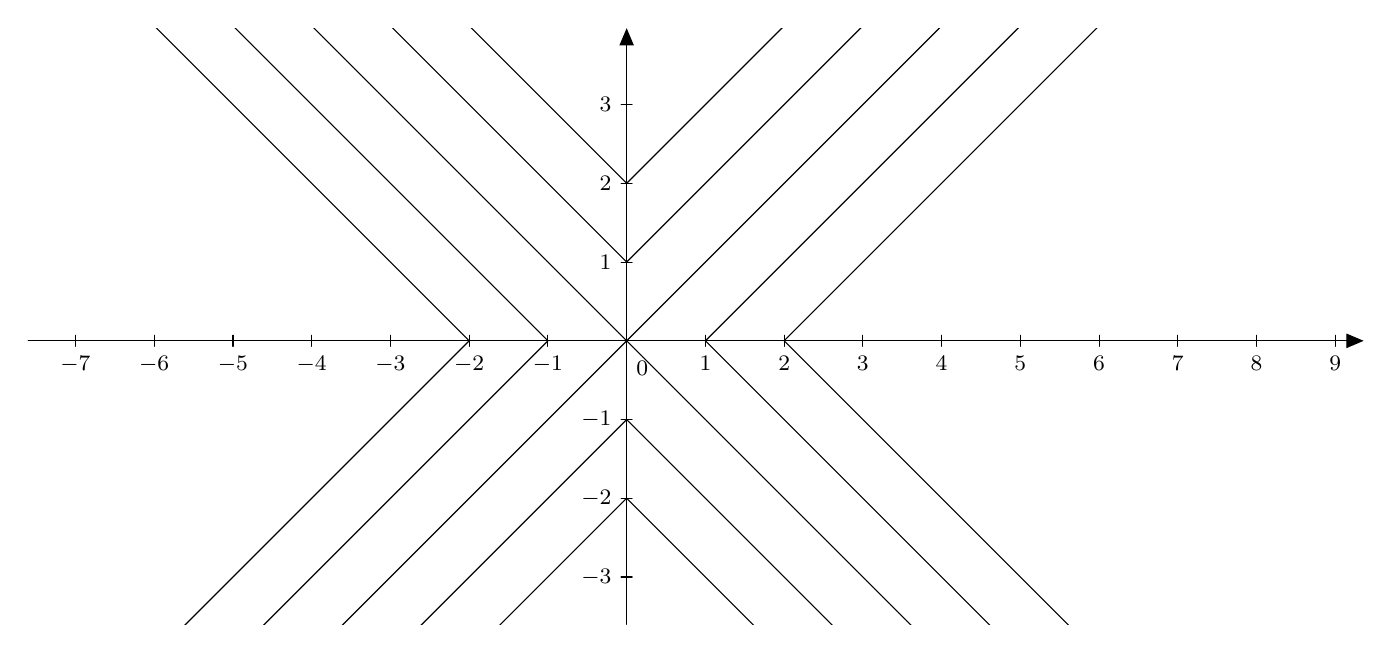
\begin{tikzpicture}[line cap=round,line join=round,>=triangle 45,x=1.0cm,y=1.0cm]
\draw[->,color=black] (-7.6,0) -- (9.36,0);
\foreach \x in {-7,-6,-5,-4,-3,-2,-1,1,2,3,4,5,6,7,8,9}
\draw[shift={(\x,0)},color=black] (0pt,2pt) -- (0pt,-2pt) node[below] {\footnotesize $\x$};
\draw[->,color=black] (0,-3.6) -- (0,3.97);
\foreach \y in {-3,-2,-1,1,2,3}
\draw[shift={(0,\y)},color=black] (2pt,0pt) -- (-2pt,0pt) node[left] {\footnotesize $\y$};
\draw[color=black] (0pt,-10pt) node[right] {\footnotesize $0$};
\clip(-7.6,-3.6) rectangle (9.36,3.97);
\draw [domain=0.0:9.36317978586575] plot(\x,{(-0--1*\x)/1});
\draw [domain=0.0:9.36317978586575] plot(\x,{(--1--1*\x)/1});
\draw [domain=0.0:9.36317978586575] plot(\x,{(--2--1*\x)/1});
\draw [domain=1.0:9.36317978586575] plot(\x,{(-1--1*\x)/1});
\draw [domain=2.0:9.36317978586575] plot(\x,{(-2--1*\x)/1});
\draw [domain=0.0:9.36317978586575] plot(\x,{(-2-1*\x)/1});
\draw [domain=0.0:9.36317978586575] plot(\x,{(-1-1*\x)/1});
\draw [domain=0.0:9.36317978586575] plot(\x,{(-0-1*\x)/1});
\draw [domain=1.0:9.36317978586575] plot(\x,{(--1-1*\x)/1});
\draw [domain=2.0:9.36317978586575] plot(\x,{(--2-1*\x)/1});
\draw [domain=-7.600390760110365:0.0] plot(\x,{(-0-1*\x)/-1});
\draw [domain=-7.600390760110365:-2.0] plot(\x,{(-2-1*\x)/-1});
\draw [domain=-7.600390760110365:-1.0] plot(\x,{(-1-1*\x)/-1});
\draw [domain=-7.600390760110365:0.0] plot(\x,{(--1-1*\x)/-1});
\draw [domain=-7.600390760110365:0.0] plot(\x,{(--2-1*\x)/-1});
\draw [domain=-7.600390760110365:-2.0] plot(\x,{(--2--1*\x)/-1});
\draw [domain=-7.600390760110365:-1.0] plot(\x,{(--1--1*\x)/-1});
\draw [domain=-7.600390760110365:0.0] plot(\x,{(-0--1*\x)/-1});
\draw [domain=-7.600390760110365:0.0] plot(\x,{(-1--1*\x)/-1});
\draw [domain=-7.600390760110365:0.0] plot(\x,{(-2--1*\x)/-1});
\end{tikzpicture}
显然该微分方程的奇异点都在横纵坐标轴上.
\end{proof}
\begin{exercise}[习题1-2,1,(2)]
作出如下微分方程的线素场:$y'=(y-1)^2$.  
\end{exercise}
\begin{proof}[解]
我们先求线素场的等斜线.令 $y'=(y-1)^2=k$,则
\begin{equation}
  \label{eq:3.09pm}
  y=\pm\sqrt{k}+1.
\end{equation}
这说明线素斜率为 $k$ 的所有点,都是由直线 $y=\pm\sqrt{k}+1$ 组成的.当
$y>1$ 时,随着 $y$ 的增大,$y'$ 随之增大的速度更快,且 $y'$ 保持正.当
$0<y<1$ 时,随着 $y$ 的增大,$y'$ 随之减小,但是 $y'$ 仍然为正.且 $y'\in
(0,1)$.当 $y<0$ 时,随着 $y$ 的减小,$y'$ 却随之增大,且增大速度比 $y$ 的
减小速度快.如下图,短斜线就粗略地代表了线素场.\\

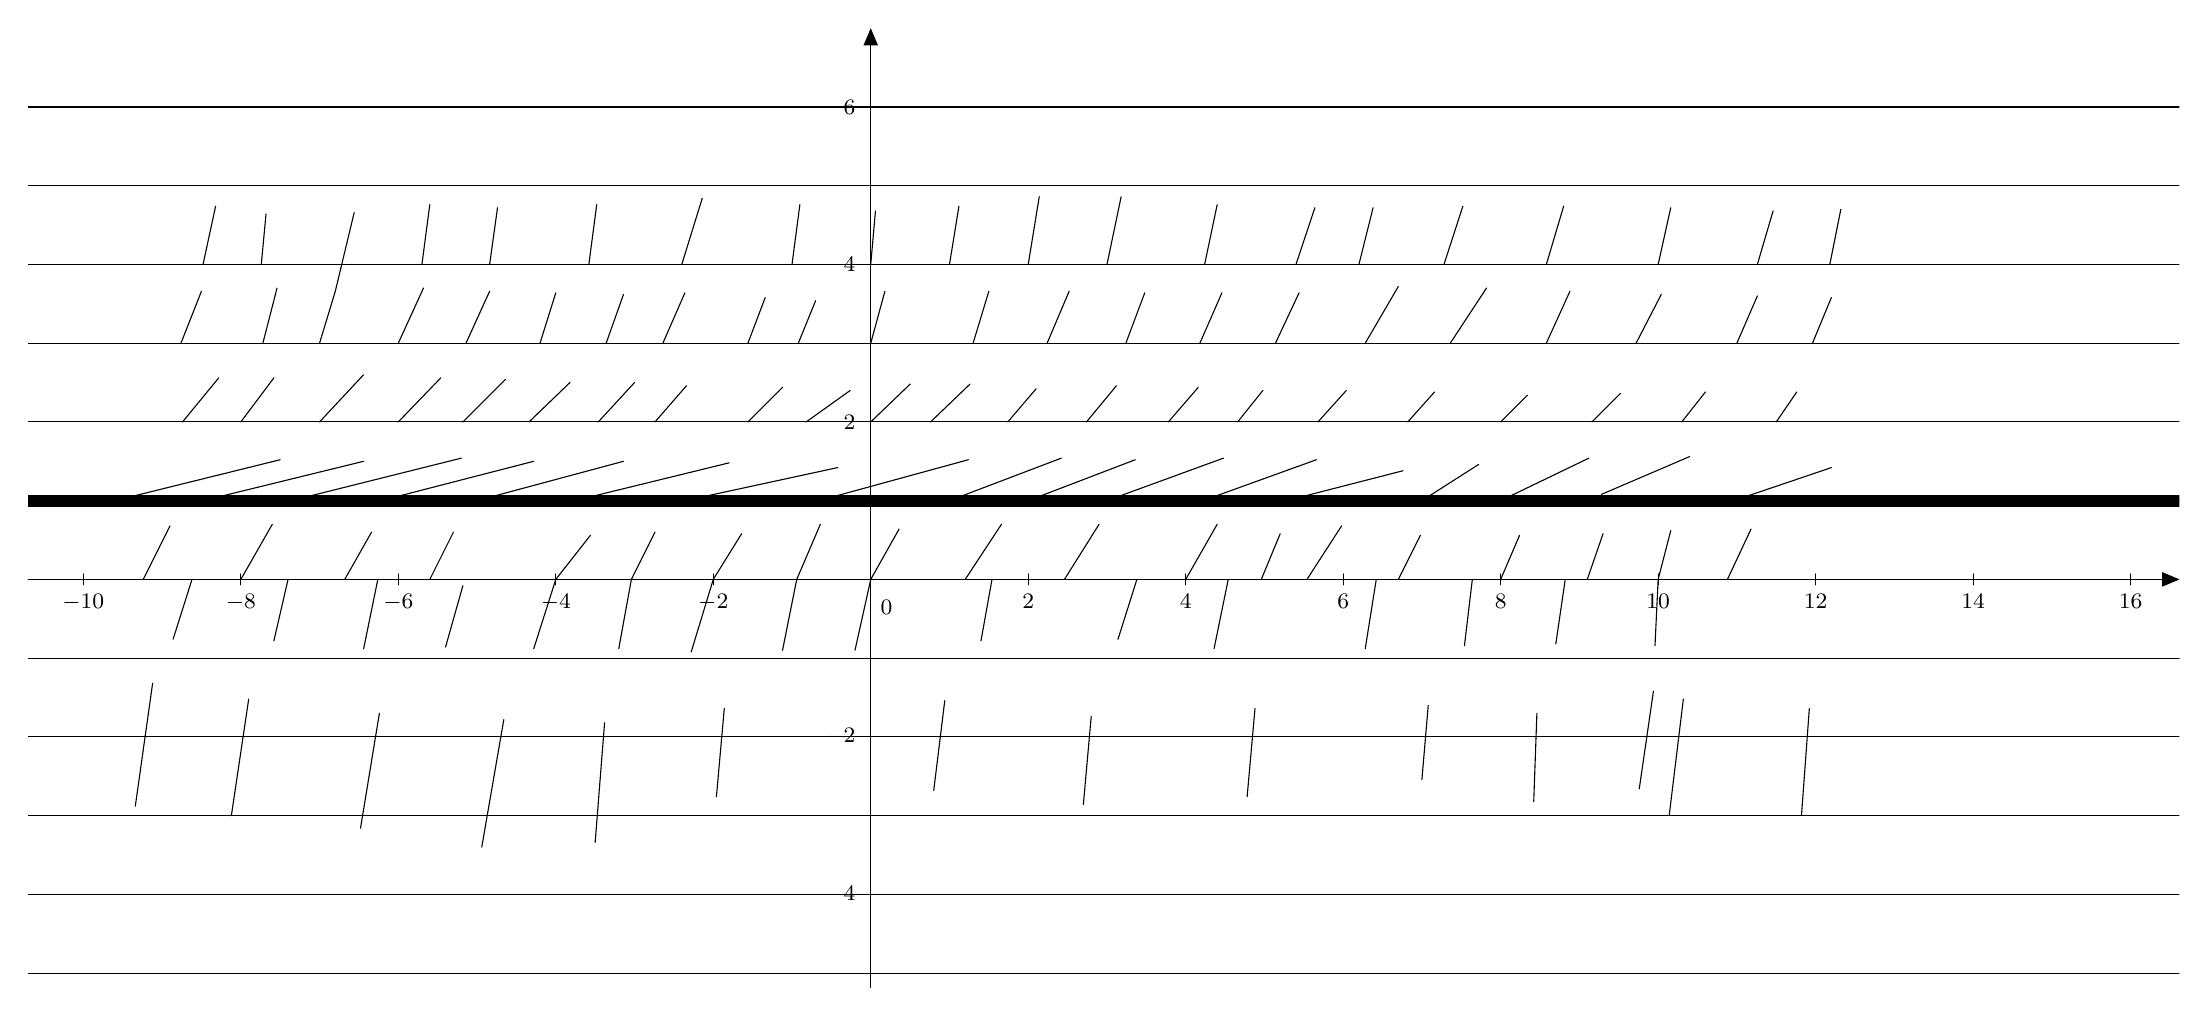
\begin{tikzpicture}[line cap=round,line join=round,>=triangle 45,x=1.0cm,y=1.0cm]
\draw[->,color=black] (-10.7,0) -- (16.62,0);
\foreach \x in {-10,-8,-6,-4,-2,2,4,6,8,10,12,14,16}
\draw[shift={(\x,0)},color=black] (0pt,2pt) -- (0pt,-2pt) node[below] {\footnotesize $\x$};
\draw[->,color=black] (0,-5.18) -- (0,7);
\foreach \y in {-4,-2,2,4,6}
\draw[shift={(0,\y)},color=black] (2pt,0pt) -- (-2pt,0pt) node[left] {\footnotesize $\y$};
\draw[color=black] (0pt,-10pt) node[right] {\footnotesize $0$};
\clip(-10.7,-5.18) rectangle (16.62,7);
\draw [domain=-10.7:16.62] plot(\x,{(--1-0*\x)/1});
\draw [domain=-10.7:16.62] plot(\x,{(--2-0*\x)/1});
\draw [domain=-10.7:16.62] plot(\x,{(--3-0*\x)/1});
\draw [domain=-10.7:16.62] plot(\x,{(--4-0*\x)/1});
\draw [domain=-10.7:16.62] plot(\x,{(--5-0*\x)/1});
\draw [domain=-10.7:16.62] plot(\x,{(--6-0*\x)/1});
\draw [domain=-10.7:16.62] plot(\x,{(-1-0*\x)/1});
\draw [domain=-10.7:16.62] plot(\x,{(-2-0*\x)/1});
\draw [domain=-10.7:16.62] plot(\x,{(-3-0*\x)/1});
\draw [domain=-10.7:16.62] plot(\x,{(-4-0*\x)/1});
\draw [domain=-10.7:16.62] plot(\x,{(-5-0*\x)/1});
\draw [line width=4.4pt,domain=-10.7:16.62] plot(\x,{(--8.62-0*\x)/8.62});
\draw [line width=0.4pt,domain=-10.7:16.62] plot(\x,{(-8.66-0*\x)/8.66});
\draw (0,2)-- (0.5,2.48);
\draw (0.76,2)-- (1.26,2.48);
\draw (1.74,2)-- (2.1,2.42);
\draw (2.74,2)-- (3.12,2.46);
\draw (3.78,2)-- (4.16,2.44);
\draw (4.66,2)-- (4.98,2.4);
\draw (5.68,2)-- (6.04,2.4);
\draw (6.82,2)-- (7.16,2.38);
\draw (8,2)-- (8.34,2.34);
\draw (9.16,2)-- (9.52,2.36);
\draw (10.3,2)-- (10.6,2.38);
\draw (11.5,2)-- (11.76,2.38);
\draw (-1.56,2)-- (-1.12,2.44);
\draw (-2.74,2)-- (-2.34,2.46);
\draw (-4.34,2)-- (-3.82,2.5);
\draw (-3.46,2)-- (-3,2.5);
\draw (-5.18,2)-- (-4.64,2.54);
\draw (-6,2)-- (-5.46,2.56);
\draw (-7,2)-- (-6.44,2.6);
\draw (-8,2)-- (-7.58,2.56);
\draw (-8.74,2)-- (-8.28,2.56);
\draw (11.96,3)-- (12.2,3.58);
\draw (11,3)-- (11.26,3.6);
\draw (9.72,3)-- (10.04,3.62);
\draw (8.58,3)-- (8.88,3.66);
\draw (7.36,3)-- (7.82,3.7);
\draw (6.28,3)-- (6.7,3.72);
\draw (5.14,3)-- (5.44,3.64);
\draw (4.18,3)-- (4.46,3.64);
\draw (3.24,3)-- (3.48,3.64);
\draw (2.24,3)-- (2.52,3.66);
\draw (1.3,3)-- (1.5,3.66);
\draw (0,3)-- (0.18,3.66);
\draw (-1.56,3)-- (-1.34,3.58);
\draw (-2.64,3)-- (-2.36,3.64);
\draw (-3.36,3)-- (-3.14,3.62);
\draw (-4.2,3)-- (-4,3.64);
\draw (-5.14,3)-- (-4.84,3.66);
\draw (-6,3)-- (-5.68,3.7);
\draw (-7,3)-- (-6.8,3.66);
\draw (-7.72,3)-- (-7.54,3.7);
\draw (-8.76,3)-- (-8.5,3.66);
\draw (12.18,4)-- (12.32,4.7);
\draw (11.26,4)-- (11.46,4.68);
\draw (10,4)-- (10.16,4.72);
\draw (8.58,4)-- (8.8,4.74);
\draw (7.28,4)-- (7.52,4.74);
\draw (6.2,4)-- (6.38,4.72);
\draw (5.4,4)-- (5.64,4.72);
\draw (4.24,4)-- (4.4,4.76);
\draw (3,4)-- (3.18,4.86);
\draw (2,4)-- (2.14,4.86);
\draw (1,4)-- (1.12,4.74);
\draw (-1,4)-- (-0.9,4.76);
\draw (-2.4,4)-- (-2.14,4.84);
\draw (-3.58,4)-- (-3.48,4.76);
\draw (-4.84,4)-- (-4.74,4.72);
\draw (-5.7,4)-- (-5.6,4.76);
\draw (-6.8,3.66)-- (-6.56,4.66);
\draw (-7.74,4)-- (-7.68,4.64);
\draw (-8.48,4)-- (-8.32,4.74);
\draw (9.28,1.08)-- (10.4,1.56);
\draw (8,1)-- (9.12,1.54);
\draw (7,1)-- (7.72,1.46);
\draw (5.28,1)-- (6.76,1.38);
\draw (4.22,1)-- (5.66,1.52);
\draw (3,1)-- (4.48,1.54);
\draw (2,1)-- (3.36,1.52);
\draw (1,1)-- (2.42,1.54);
\draw (-0.66,1)-- (1.24,1.52);
\draw (-2.36,1)-- (-0.42,1.42);
\draw (-3.76,1)-- (-1.8,1.48);
\draw (-5,1)-- (-3.14,1.5);
\draw (-6.22,1)-- (-4.28,1.5);
\draw (-7.36,1)-- (-5.2,1.54);
\draw (-8.48,1)-- (-6.44,1.5);
\draw (-9.6,1)-- (-7.5,1.52);
\draw (-0.92,3)-- (-0.7,3.54);
\draw (-0.82,2)-- (-0.26,2.4);
\draw (0,4)-- (0.06,4.68);
\draw (10.96,1)-- (12.2,1.42);
\draw (-4,0)-- (-3.56,0.56);
\draw (-2,0)-- (-1.64,0.58);
\draw (0,0)-- (0.36,0.64);
\draw (1.2,0)-- (1.66,0.7);
\draw (2.46,0)-- (2.9,0.7);
\draw (4,0)-- (4.4,0.7);
\draw (5.54,0)-- (5.98,0.68);
\draw (-0.94,0)-- (-0.64,0.7);
\draw (-3.04,0)-- (-2.74,0.6);
\draw (4.96,0)-- (5.2,0.58);
\draw (6.7,0)-- (6.98,0.56);
\draw (8,0)-- (8.24,0.56);
\draw (9.1,0)-- (9.3,0.58);
\draw (10,0)-- (10.16,0.62);
\draw (10.88,0)-- (11.18,0.64);
\draw (-5.6,0)-- (-5.3,0.6);
\draw (-6.68,0)-- (-6.34,0.6);
\draw (-8,0)-- (-7.6,0.7);
\draw (-9.24,0)-- (-8.9,0.68);
\draw (-4,0)-- (-4.28,-0.88);
\draw (-3.04,0)-- (-3.2,-0.88);
\draw (-2,0)-- (-2.28,-0.92);
\draw (-0.94,0)-- (-1.12,-0.9);
\draw (0,0)-- (-0.2,-0.9);
\draw (1.54,0)-- (1.4,-0.78);
\draw (3.38,0)-- (3.14,-0.76);
\draw (4.54,0)-- (4.36,-0.88);
\draw (6.42,0)-- (6.28,-0.88);
\draw (7.64,0)-- (7.54,-0.84);
\draw (8.82,0)-- (8.7,-0.82);
\draw (10,0)-- (9.96,-0.84);
\draw (-5.18,-0.08)-- (-5.4,-0.86);
\draw (-6.26,0)-- (-6.44,-0.88);
\draw (-7.4,0)-- (-7.58,-0.78);
\draw (-8.62,0)-- (-8.86,-0.76);
\draw (-9.12,-1.32)-- (-9.34,-2.88);
\draw (-7.9,-1.52)-- (-8.12,-3);
\draw (-6.24,-1.7)-- (-6.48,-3.16);
\draw (-4.66,-1.78)-- (-4.94,-3.4);
\draw (-3.38,-1.82)-- (-3.5,-3.34);
\draw (-1.86,-1.64)-- (-1.96,-2.76);
\draw (0.94,-1.54)-- (0.8,-2.68);
\draw (2.8,-1.74)-- (2.7,-2.86);
\draw (4.88,-1.64)-- (4.78,-2.76);
\draw (7.08,-1.6)-- (7,-2.54);
\draw (8.46,-1.7)-- (8.42,-2.82);
\draw (9.76,-2.66)-- (9.94,-1.42);
\draw (10.32,-1.52)-- (10.14,-3);
\draw (11.92,-1.64)-- (11.82,-3);
\end{tikzpicture}

为了验证,我们用 matlab 作一下图.代码如下:

\begin{lstlisting}
>> [x,y]=meshgrid(-3:.5:3,-3:.5:3);
>> dy=(y-1).^2;
>> dx=ones(size(dy));
>> dyu=dy./sqrt(dy.^2+dx.^2);
>> dxu=dx./sqrt(dy.^2+dx.^2);
>> quiver(x,y,dxu,dyu)
\end{lstlisting}
最后出来的效果是\\
\includegraphics[width=1\textwidth]{/home/luqing/vectorfield1.png}
可见,虽然我自己的图画的烂了一点,但是还是基本正确的.显然,该方程没有奇点.
\end{proof}
\begin{exercise}[习题1-2,(3)]
作出如下微分方程的线素场:$y'=x^2+y^2$.  
\end{exercise}
\begin{proof}[解]
我们先做出线素场的等斜线.令
$$
y'=x^2+y^2=k,
$$
则可得斜率为 $k$ 的所有点组成以原点为圆心的,半径为 $\sqrt{k}$ 的圆.当
圆的半径越来越大时,那些点的斜率以快的多的速度增长.我们用 matlab 画图,代码是
\begin{lstlisting}
>> [x,y]=meshgrid(-3:.5:3,-3:.5:3);
>> dy=x.^2+y.^2;
>> dx=ones(size(dy));
>> dyu=dy./sqrt(dy.^2+dx.^2);
>> dxu=dx./sqrt(dy.^2+dx.^2);
>> quiver(x,y,dxu,dyu)
\end{lstlisting}
得到线素场\\
\includegraphics[width=1\textwidth]{/home/luqing/vectorfield2.png}
\end{proof}
\begin{exercise}[习题1-2,2,(1)]
利用线素场研究微分方程 $y'=1+xy$  的积分曲线族.
\end{exercise}
\begin{proof}[解]
  该微分方程的线素场的等斜线是
$$
y'=1+xy=k.
$$
得到
$$
xy=k-1.
$$
当 $k=1$ 时,$x=0$ 或 $y=0$ 是等斜线,积分曲线位于 $x=0,y=0$ 上的点的斜率都为1.用 matlab 画线素场的代码如下
\begin{lstlisting}
>> [x,y]=meshgrid(-3:.5:3,-3:.5:3);
>> dy=1+x.*y;
>> dx=ones(size(dy));
>> dyu=dy./sqrt(dy.^2+dx.^2);
>> dxu=dx./sqrt(dy.^2+dx.^2);
>> quiver(x,y,dxu,dyu)
\end{lstlisting}
线素场图像如下:\\
\includegraphics[width=1\textwidth]{/home/luqing/vectorfield3.png}
该微分方程没有奇点.
\end{proof}
\begin{exercise}[习题1-2,2,(2)]
  利用线素场研究微分方程 $y'=x^2-y^2$ 的积分曲线族.
\end{exercise}
\begin{proof}[解]
先求该微分方程的等斜线.令
$$
y'=x^2-y^2=k,
$$
其中 $k$ 是常数.当 $k=0$ 时,得到等斜线 $x=\pm y$,可见,等斜线 $x=y$ 和
$x=-y$ 上的点斜率都为 0.当 $k>0$ 时,等斜线(双曲线)$x^2-y^2=k$ 的极径是沿着横
坐标方向的,当 $k<0$ 时,等斜线(双曲线) $x^2-y^2=k$ 的极径是沿着纵坐标方向的.用 matlab 画出线素场,代码如下:
 \begin{lstlisting}
>> [x,y]=meshgrid(-3:.5:3,-3:.5:3);
>> dy=x.^2-y.^2;
>> dx=ones(size(dy));
>> dyu=dy./sqrt(dy.^2+dx.^2);
>> dxu=dx./sqrt(dy.^2+dx.^2);
>> quiver(x,y,dxu,dyu)
 \end{lstlisting}
图像如下\\
\includegraphics[width=1\textwidth]{/home/luqing/vectorfield4.png}
该微分方程没有奇点.
\end{proof}
\end{document}
